\documentclass[11pt]{article}

\usepackage[T1]{fontenc}
\usepackage[utf8]{inputenc}
\usepackage[spanish,es-noshorthands]{babel}
\usepackage{amsmath,amssymb}
\usepackage{graphicx}
\usepackage[margin=2.5cm]{geometry}
\usepackage{algorithm}
\usepackage{algpseudocode}
\usepackage{booktabs}
\usepackage{float}
\usepackage{listings}
\usepackage{url}
\usepackage{xcolor}
\usepackage[hidelinks]{hyperref}

% --- Pseudocódigo en español -------------------------------------------------
\floatname{algorithm}{Algoritmo}
\algrenewcommand\algorithmicrequire{\textbf{Entrada:}}
\algrenewcommand\algorithmicensure{\textbf{Salida:}}
\algrenewcommand\algorithmicfor{\textbf{para}}
\algrenewcommand\algorithmicforall{\textbf{para todo}}
\algrenewcommand\algorithmicdo{\textbf{hacer}}
\algrenewcommand\algorithmicwhile{\textbf{mientras}}
\algrenewcommand\algorithmicif{\textbf{si}}
\algrenewcommand\algorithmicthen{\textbf{entonces}}
\algrenewcommand\algorithmicelse{\textbf{si no}}
\algrenewcommand\algorithmicend{\textbf{fin}}
\algrenewcommand\algorithmicreturn{\textbf{retornar}}

% --- Estilo para código C++ ---------------------------------------------------
\lstdefinestyle{cpp}{
  language=C++,
  basicstyle=\ttfamily\footnotesize,
  keywordstyle=\color{blue!70!black}\bfseries,
  commentstyle=\color{gray!60!black}\itshape,
  stringstyle=\color{orange!70!black},
  numbers=left,
  numberstyle=\tiny\color{gray},
  numbersep=8pt,
  breaklines=true,
  showstringspaces=false,
  frame=single,
  framerule=0.3pt,
  tabsize=4
}
\lstdefinestyle{texto}{
  basicstyle=\ttfamily\footnotesize,
  frame=single,
  framerule=0.3pt
}

\title{Tarea 2\\[2mm] \large 501404, 503309 --- Análisis de Algoritmos}
\author{Erick Saldivar \and Alejandro Neira}
\date{Fecha de entrega: lunes 6 de julio de 2026}

\begin{document}
\maketitle

\section{Diseño}

\paragraph{Notación.}
$G=(V,E)$ es un grafo dirigido con pesos $w\colon E\to\mathbb{R}$,
$n:=|V|$ y $m:=|E|$. Un \emph{camino} de $u$ a $v$ es una secuencia
$p=\langle v_0,\dots,v_\ell\rangle$ con $v_0=u$, $v_\ell=v$ y
$(v_{i-1},v_i)\in E$; su peso es $w(p)=\sum_{i=1}^{\ell}w(v_{i-1},v_i)$, es
\emph{simple} si no repite vértices y sus \emph{vértices intermedios} son
$v_1,\dots,v_{\ell-1}$. La distancia mínima es
$\delta(u,v):=\inf\{w(p):p\text{ camino de }u\text{ a }v\}$, con valor
$+\infty$ si no existe camino, y el problema APSP consiste en calcular
$\delta(u,v)$ para todo par $(u,v)\in V\times V$. Si $G$ contiene un ciclo
de peso negativo, las distancias a través de él no están bien definidas
(recorriéndolo el peso decrece sin cota); suponemos que no los hay, y ambos
algoritmos detectan y reportan esta situación cuando ocurre.

\subsection{Algoritmo Base: APSP mediante $n$ llamadas a Bellman-Ford}
\label{sec:base}

El algoritmo de Bellman-Ford, visto en clases, resuelve el problema del
camino más corto con \emph{una} fuente (SSSP): dado $s\in V$, calcula
$\delta(s,v)$ para todos los $v\in V$ a la vez, relajando las $m$ aristas
durante $n-1$ rondas, y con una ronda adicional detecta si existe algún
ciclo negativo alcanzable desde $s$ \cite[cap.~24]{clrs}. Las $n-1$ rondas
bastan porque, sin ciclos negativos, los caminos más cortos pueden tomarse
\emph{simples} (a lo más $n-1$ aristas): eliminar de un camino un ciclo, de
peso $\ge 0$, no aumenta su peso.

\textbf{Argumento.} La solución de APSP es la matriz $D$ de $n\times n$
definida por $D[u][v]=\delta(u,v)$. Su fila $u$, es decir la familia de
valores $(\delta(u,v))_{v\in V}$, es \emph{exactamente} la salida del
problema SSSP con fuente $u$, que una llamada $\textsc{BellmanFord}(G,w,u)$
calcula correctamente. Como las $n$ filas cubren todos los pares de
$V\times V$, basta ejecutar Bellman-Ford una vez por cada $u\in V$ para
obtener la matriz completa: $n$ llamadas resuelven APSP. El procedimiento
resultante es el \emph{Algoritmo Base} (Algoritmo~\ref{alg:base}). Nótese
además que todo ciclo negativo es alcanzable desde sus propios vértices y
que el Algoritmo Base ejecuta Bellman-Ford desde \emph{todas} las fuentes,
por lo que detecta cualquier ciclo negativo de $G$.

\begin{algorithm}[ht]
\caption{\textsc{AlgoritmoBase}$(G,w)$}\label{alg:base}
\begin{algorithmic}[1]
\Require grafo dirigido $G=(V,E)$ con pesos $w$
\Ensure matriz $D$ con $D[u][v]=\delta(u,v)$ para todo $(u,v)\in V\times V$
\For{cada $u\in V$}
  \State $D[u][\,\cdot\,]\gets\textsc{BellmanFord}(G,w,u)$
\EndFor
\State \Return $D$
\end{algorithmic}
\end{algorithm}

\textbf{Análisis de complejidad.} Cada llamada a Bellman-Ford ejecuta a lo
más $n$ rondas ($n-1$ de relajación más la de detección), cada una con
trabajo $O(1)$ por arista; junto con la inicialización, una llamada cuesta
$O(n+nm)=O(nm)$. El Algoritmo Base realiza $n$ llamadas, para un total de
\[
O(n^2 m).
\]
En grafos \emph{densos} ($m=\Theta(n^2)$) esto es $O(n^4)$; en grafos
\emph{dispersos} ($m=O(n)$), $O(n^3)$. El espacio es $\Theta(n^2)$: el
tamaño de la propia salida, más $O(n)$ auxiliar por llamada (el vector de
distancias).

\subsection{Algoritmo de Floyd-Warshall}
\label{sec:fw}

Diseñamos un algoritmo de programación dinámica que resuelve APSP en tiempo
$\Theta(n^3)$, sin depender de $m$. Identificamos los vértices con los
enteros $V=\{1,2,\dots,n\}$.

\textbf{Subproblemas.} La dificultad de APSP está en que un camino más
corto de $i$ a $j$ puede pasar por cualquier subconjunto de vértices. La
idea es \emph{restringir qué vértices pueden usarse como intermedios} e ir
liberando la restricción gradualmente: para $0\le k\le n$, sea
$V_k:=\{1,\dots,k\}$ (con $V_0=\emptyset$) y
\[
\delta^{(k)}(i,j)\;:=\;\inf\{\,w(p) : p\text{ es un camino de } i\text{ a } j
\text{ con todos sus vértices intermedios en } V_k\,\},
\]
con valor $+\infty$ si no existe tal camino; los \emph{extremos} $i,j$ no
están restringidos. Como $V_n=V$ no impone restricción alguna,
$\delta^{(n)}=\delta$: resolver los subproblemas de nivel $n$ resuelve APSP.
Notemos que, sin ciclos negativos, todo camino se transforma en uno
\emph{simple} de peso menor o igual eliminando ciclos (cada uno de peso
$\ge 0$) y sin agregar intermedios nuevos; el ínfimo se alcanza entonces en
un camino simple, y en particular $\delta^{(k)}(u,u)=0$ para todo $u,k$.

\textbf{Recurrencia.} Sea $k\ge 1$ y sea $p$ un camino más corto de $i$ a
$j$ con intermedios en $V_k$, tomado simple. Hay exactamente dos casos:
\begin{itemize}
  \item \emph{$k$ no es intermedio de $p$}: todos los intermedios de $p$
  están en $V_{k-1}$, y $p$ es candidato del subproblema de nivel $k-1$;
  \item \emph{$k$ es intermedio de $p$}: como $p$ es simple, $k$ aparece
  exactamente una vez y descompone a $p$ en $p_1\colon i\to k$ y
  $p_2\colon k\to j$, ambos con intermedios en $V_{k-1}$. Por la
  subestructura óptima de los caminos más cortos (vista en clases: todo
  subcamino de un camino más corto es un camino más corto entre sus
  extremos, pues si hubiera uno mejor, sustituirlo daría un camino total
  mejor), $p_1$ y $p_2$ son óptimos en sus subproblemas de nivel $k-1$.
\end{itemize}
Esto motiva definir los valores de programación dinámica
\begin{equation}\label{eq:recurrencia}
D^{(0)}_{ij}=
\begin{cases}
0 & \text{si } i=j,\\
w(i,j) & \text{si } i\ne j \text{ y } (i,j)\in E,\\
+\infty & \text{en otro caso,}
\end{cases}
\qquad
D^{(k)}_{ij}=\min\Bigl(D^{(k-1)}_{ij},\; D^{(k-1)}_{ik}+D^{(k-1)}_{kj}\Bigr)
\end{equation}
para $1\le k\le n$. (Con aristas paralelas $(i,j)$, en $D^{(0)}_{ij}$ se
toma la de menor peso.)

\textbf{Correctitud.} Probamos por inducción sobre $k$ que
$D^{(k)}_{ij}=\delta^{(k)}(i,j)$ para todo par $(i,j)$; con $k=n$ esto da
$D^{(n)}_{ij}=\delta(i,j)$. Caso base $k=0$: un camino sin intermedios es el
camino trivial $\langle i\rangle$ (solo si $i=j$, de peso $0$; un lazo
$(i,i)$ de peso menor sería un ciclo negativo) o una única arista $(i,j)$,
y $D^{(0)}_{ij}$ toma el mínimo entre estas posibilidades. Paso inductivo:
supongamos $D^{(k-1)}=\delta^{(k-1)}$.
$(\ge)$ Cada argumento finito del mínimo en \eqref{eq:recurrencia} es el
peso de un camino real de $i$ a $j$ con intermedios en $V_k$: el primero, de
un camino con intermedios en $V_{k-1}\subseteq V_k$; el segundo, de la
concatenación de caminos óptimos $i\to k$ y $k\to j$ con intermedios en
$V_{k-1}$ (la concatenación puede repetir vértices, pero sigue siendo un
camino). Luego $D^{(k)}_{ij}\ge\delta^{(k)}(i,j)$.
$(\le)$ Sea $p$ un camino más corto (simple) de $i$ a $j$ con intermedios en
$V_k$; por el análisis de casos de la recurrencia, si $k$ no es intermedio
de $p$ entonces $D^{(k)}_{ij}\le D^{(k-1)}_{ij}=\delta^{(k-1)}(i,j)\le w(p)$,
y si $k$ es intermedio entonces
$D^{(k)}_{ij}\le D^{(k-1)}_{ik}+D^{(k-1)}_{kj}=w(p_1)+w(p_2)=w(p)$. En ambos
casos $D^{(k)}_{ij}\le\delta^{(k)}(i,j)$, lo que completa la inducción.

\textbf{Algoritmo.} La recurrencia puede evaluarse sobre una \emph{única}
matriz $D$ actualizada in situ. En efecto, como
$D^{(k-1)}_{kk}=\delta^{(k-1)}(k,k)=0$, la etapa $k$ deja invariantes la
fila y la columna $k$:
$D^{(k)}_{ik}=\min(D^{(k-1)}_{ik},D^{(k-1)}_{ik}+0)=D^{(k-1)}_{ik}$ y
simétricamente $D^{(k)}_{kj}=D^{(k-1)}_{kj}$; y esas son exactamente las
entradas que la etapa $k$ lee. El resultado es el algoritmo de
Floyd-Warshall (Algoritmo~\ref{alg:fw}).

\begin{algorithm}[ht]
\caption{\textsc{FloydWarshall}$(G,w)$}\label{alg:fw}
\begin{algorithmic}[1]
\Require grafo dirigido $G=(V,E)$ con pesos $w$, $V=\{1,\dots,n\}$
\Ensure matriz $D$ con $D[i][j]=\delta(i,j)$, o reporte de ciclo negativo
\State $D[i][j]\gets 0$ si $i=j$;\; $w(i,j)$ si $(i,j)\in E$;\; $\infty$ en otro caso \Comment{$D=D^{(0)}$}
\For{$k\gets 1$ \textbf{hasta} $n$}
  \For{$i\gets 1$ \textbf{hasta} $n$}
    \For{$j\gets 1$ \textbf{hasta} $n$}
      \If{$D[i][k]+D[k][j]<D[i][j]$}
        \State $D[i][j]\gets D[i][k]+D[k][j]$
      \EndIf
    \EndFor
  \EndFor
\EndFor
\If{$D[i][i]<0$ para algún $i\in V$}
  \State \textbf{reportar} ciclo negativo
\EndIf
\State \Return $D$
\end{algorithmic}
\end{algorithm}

\textbf{Detección de ciclos negativos.} La comprobación final del
Algoritmo~\ref{alg:fw} es correcta: al terminar existe $D[i][i]<0$ si y solo
si $G$ contiene un ciclo negativo. $(\Rightarrow)$ Toda entrada finita de
$D$ es en todo momento el peso de un camino real (vale al inicializar, y
cada actualización concatena dos caminos reales $i\to k$ y $k\to j$); si
$D[i][i]<0$ existe un camino cerrado de peso negativo, y como todo camino
cerrado se descompone en ciclos simples, alguno de ellos es negativo.
$(\Leftarrow)$ La desigualdad $(\le)$ de la correctitud vale \emph{sin
hipótesis sobre ciclos}: tras la etapa $k$, $D[i][j]\le w(p)$ para todo
camino simple $p$ de $i$ a $j$ con intermedios en $V_k$ (misma inducción,
usando que las entradas nunca aumentan). Sea $C$ un ciclo simple de peso
negativo. Si es un lazo $(u,u)$, la inicialización ya deja
$D[u][u]\le w(u,u)<0$. Si no, sean $x$ e $y$ sus dos vértices de mayor
índice: $y$ parte a $C$ en dos caminos simples $p_1\colon x\to y$ y
$p_2\colon y\to x$ con intermedios en $V_{y-1}$, y al procesar el par
$(x,x)$ en la etapa $k=y$ queda
$D[x][x]\le D[x][y]+D[y][x]\le w(p_1)+w(p_2)=w(C)<0$, cota que se conserva
hasta el final porque las entradas solo decrecen.

\textbf{Análisis de complejidad.} La inicialización cuesta $\Theta(n^2)$
más $O(m)$ por recorrer las aristas. El cuerpo del triple bucle realiza
trabajo $O(1)$ (una suma, una comparación y a lo más una asignación) y se
ejecuta exactamente $n^3$ veces; la revisión final de la diagonal cuesta
$O(n)$. El total es
\[
\Theta(n^3),
\]
independiente de $m$, con espacio $\Theta(n^2)$: una única matriz, que
coincide con el tamaño de la salida. Frente al Algoritmo Base ($O(n^2m)$),
en grafos densos Floyd-Warshall gana un factor $n$ completo ($\Theta(n^3)$
contra $O(n^4)$); en grafos dispersos ambos son $O(n^3)$, pero el bucle
interno de Floyd-Warshall solo hace aritmética sobre una matriz contigua en
memoria, con constantes menores. La comparación empírica es objeto de la
sección de experimentos.

\section{Implementación y verificación de correctitud (pregunta 2.1)}
\label{sec:implementacion}

\subsection{Entorno y decisiones de implementación}

Ambos algoritmos fueron implementados en \textbf{C++17}, sin emplear
librerías con subrutinas para grafos: solo se usan contenedores estándar
(\texttt{std::vector}) y utilidades de entrada/salida. El código se compila
con \texttt{g++} (GCC 16.1.0, MinGW-w64 de MSYS2) usando la opción
\texttt{-O2}. Las decisiones principales son las siguientes.

\begin{itemize}
  \item \textbf{Representación del grafo} (\texttt{src/grafo.hpp}): lista de
  aristas \texttt{Arista}~$=(u,v,w)$ con nodos $0$-indexados y pesos
  \texttt{double}. Bellman-Ford recorre precisamente la lista de aristas, y
  Floyd-Warshall solo la usa para construir $D^{(0)}$, por lo que esta
  representación sirve a ambos sin estructuras adicionales.
  \item \textbf{Infinito} : la ausencia de camino se representa con
  \texttt{INF = std::numeric\_limits<double>::infinity()}. La aritmética
  IEEE~754 garantiza $\infty+c=\infty$ e $\infty+\infty=\infty$, y que toda
  comparación $\infty+c<x$ con $x$ finito sea falsa; así las relajaciones no
  requieren casos especiales.
  \item \textbf{Bellman-Ford} (\texttt{bellman\_ford} en
  \texttt{src/apsp.hpp}): implementa el algoritmo visto en clases
  (sección~\ref{sec:base}) con una
  mejora estándar: si una ronda completa no produce ninguna relajación, el
  vector de distancias alcanzó un punto fijo y el algoritmo termina antes.
  Esto no afecta la correctitud (el punto fijo ya es la solución) pero
  reduce el tiempo en instancias favorables. La ronda extra de detección de
  ciclos negativos se realiza siempre.
  \item \textbf{Algoritmo Base} (\texttt{algoritmo\_base}): $n$ llamadas a
  \texttt{bellman\_ford}, una por fuente, exactamente como en el
  Algoritmo~\ref{alg:base}.
  \item \textbf{Floyd-Warshall} (\texttt{floyd\_warshall}): transcripción
  directa del Algoritmo~\ref{alg:fw}, con la actualización in situ
  justificada en la sección~\ref{sec:fw}. Si la entrada contiene aristas
  paralelas, en $D^{(0)}$ se conserva la de menor peso; los lazos de peso
  negativo quedan en la diagonal y son detectados como ciclos negativos.
  \item \textbf{Detección de ciclos negativos}: ambas funciones aceptan un
  puntero opcional \texttt{ciclo\_negativo} donde reportan la detección
  justificada en las secciones~\ref{sec:base} y~\ref{sec:fw}, lo que
  permite contrastar también este aspecto entre ambos algoritmos.
\end{itemize}

Las instancias se leen desde archivos de texto con el formato siguiente
(nodos $0$-indexados; una arista dirigida por línea):

\begin{lstlisting}[style=texto]
n m
u v w        (m lineas: arista u -> v con peso real w)
\end{lstlisting}

\pagebreak

\subsection{Marco comparativo para verificar la correctitud}
\label{sec:verificacion}

La verificación está automatizada en el programa \texttt{src/verificar.cpp},
que ejecuta dos baterías de pruebas y termina con código de salida $0$ solo
si todas pasan.

\paragraph{Batería 1: instancias con solución conocida.}
Cuatro instancias pequeñas cuya matriz de distancias completa se conoce de
antemano (calculada a mano o tomada de la literatura), elegidas para cubrir
modos de falla distintos. Cada algoritmo debe reproducir la matriz esperada
\emph{exactamente}, y en el caso del ciclo negativo, ambos deben detectarlo.
El Cuadro~\ref{tab:casos} resume las instancias; los archivos están en
\texttt{tests/casos/}.

\begin{table}[ht]
\centering
\begin{tabular}{lccp{5.6cm}l}
\toprule
Instancia & $n$ & $m$ & Qué verifica & Origen de la solución\\
\midrule
\texttt{caso1\_clrs} & 5 & 9 & pesos negativos sin ciclo negativo; caminos óptimos no triviales & Fig.~25.1 de \cite{clrs}\\
\texttt{caso2\_camino} & 4 & 3 & pares inalcanzables ($\infty$) en un camino dirigido & cálculo a mano\\
\texttt{caso3\_ciclo\_negativo} & 3 & 3 & detección de ciclo negativo (peso fraccionario $0.5$) & cálculo a mano\\
\texttt{caso4\_fuertemente\_conexo} & 4 & 6 & ciclos de peso positivo; aristas directas peores que caminos indirectos & cálculo a mano\\
\bottomrule
\end{tabular}
\caption{Instancias con solución conocida usadas como marco comparativo.}
\label{tab:casos}
\end{table}

\paragraph{Batería 2: verificación cruzada aleatoria.}
El Algoritmo Base y Floyd-Warshall son implementaciones independientes
basadas en técnicas distintas (relajación iterativa por aristas contra
programación dinámica sobre intermedios); que ambas coincidan entrada a
entrada sobre una colección grande y variada de instancias es evidencia
fuerte de correctitud, pues un error en cualquiera de las dos difícilmente
produciría exactamente las mismas matrices. Se generan $200$ grafos
aleatorios $G(n,p)$ reproducibles (generador \texttt{std::mt19937} con
semilla fija $20260706$), con $n$ uniforme en $[1,40]$, densidad
$p\in\{0.1,0.3,0.6,0.9\}$ rotando entre pruebas, y pesos múltiplos de $0.25$
en $[0,10]$ (pruebas pares) o en $[-3,10]$ (pruebas impares, donde pueden
aparecer ciclos negativos). Como los múltiplos de $0.25$ son exactamente
representables en \texttt{double}, las sumas de pesos son exactas y la
comparación entre ambas matrices puede exigir igualdad exacta. El criterio
de éxito por prueba es: ambos algoritmos coinciden en la detección de ciclo
negativo y, en ausencia de este, sus matrices son idénticas (con ciclo
negativo las distancias no están bien definidas y no se comparan).

\subsection{Resultados de la verificación}

La salida completa del programa es la siguiente:

\begin{lstlisting}[style=texto]
== Bateria 1: instancias con solucion conocida (tests/casos) ==
  [OK] caso1_clrs.grafo (n=5, m=9)
  [OK] caso2_camino.grafo (n=4, m=3)
  [OK] caso3_ciclo_negativo.grafo (n=3, m=3)
  [OK] caso4_fuertemente_conexo.grafo (n=4, m=6)
== Bateria 2: verificacion cruzada sobre 200 grafos aleatorios ==
  200/200 pruebas correctas (86 instancias con ciclo negativo,
  detectado por ambos algoritmos)
== RESULTADO: todas las pruebas pasaron ==
\end{lstlisting}

Las cuatro instancias conocidas son reproducidas exactamente por ambos
algoritmos, y en las $200$ instancias aleatorias ambos coinciden por
completo; en las $86$ que contienen ciclos negativos, ambos los detectan.
Las instrucciones para compilar y ejecutar la verificación están en el
archivo \texttt{README.md} del repositorio; en síntesis:

\begin{lstlisting}[style=texto]
g++ -std=c++17 -O2 -o verificar src/verificar.cpp
./verificar
\end{lstlisting}

% ==============================================================================
\section{Experimentos (pregunta 2.2)}
\label{sec:experimentos}

\subsection{Configuración experimental}

Todos los experimentos se ejecutaron en la misma máquina:
Windows~11, CPU AMD Ryzen~7~5800X (8 núcleos, 3.80~GHz), 24~GB~RAM,
compilador \texttt{g++}~16.1.0 (MinGW-w64, MSYS2), bandera \texttt{-O2}.
Las llamadas a los algoritmos se protegen con \texttt{volatile} para evitar
que el compilador las elimine del bucle de medición, incluso con
optimizaciones habilitadas. Se eligió \texttt{-O2} en lugar del
\texttt{-O0} sugerido por la suite uhr porque parte de la ventaja práctica
de Floyd-Warshall reside justamente en las optimizaciones que habilita el
compilador: su acceso secuencial a una matriz contigua permite excelente
localidad de caché, loop unrolling y register allocation; medir con
\texttt{-O0} habría eliminado artificialmente estas ventajas y distorsionado
la comparación. Cada punto se midió con al menos 32 ejecuciones; los archivos CSV de salida contienen la media,
la desviación estándar y los cinco cuartiles ($Q_0,\dots,Q_4$) en
microsegundos. La semilla del generador aleatorio es fija ($20260706$) para
garantizar reproducibilidad. 

Se diseñaron cuatro experimentos que varían sistemáticamente la estructura
del grafo, cubriendo los dos extremos del espectro de densidad y la presencia
de pesos negativos. En todos los casos ambos algoritmos fueron ejecutados
sobre exactamente el mismo grafo (verificación cruzada interna dentro de cada
experimento).

\pagebreak

\subsection{Experimento 1: $n$ creciente con densidad fija}

\textbf{Parámetros:} $p=0.3$ (densidad de aristas fija), pesos en $[0,10]$,
$n\in[10,300]$ con step $10$, 64~runs por punto.

Con $p=0.3$, $m\approx 0.3\,n(n-1)=\Theta(n^2)$: el grafo es moderadamente
denso. La teoría predice $t_{\text{FW}}=\Theta(n^3)$ y
$t_{\text{Base}}=\Theta(n^2m)=\Theta(n^4)$. La Figura~\ref{fig:e1} muestra
los resultados. El código fuente está en el Anexo~\ref{app:exp1}.

\begin{figure}[H]
\centering
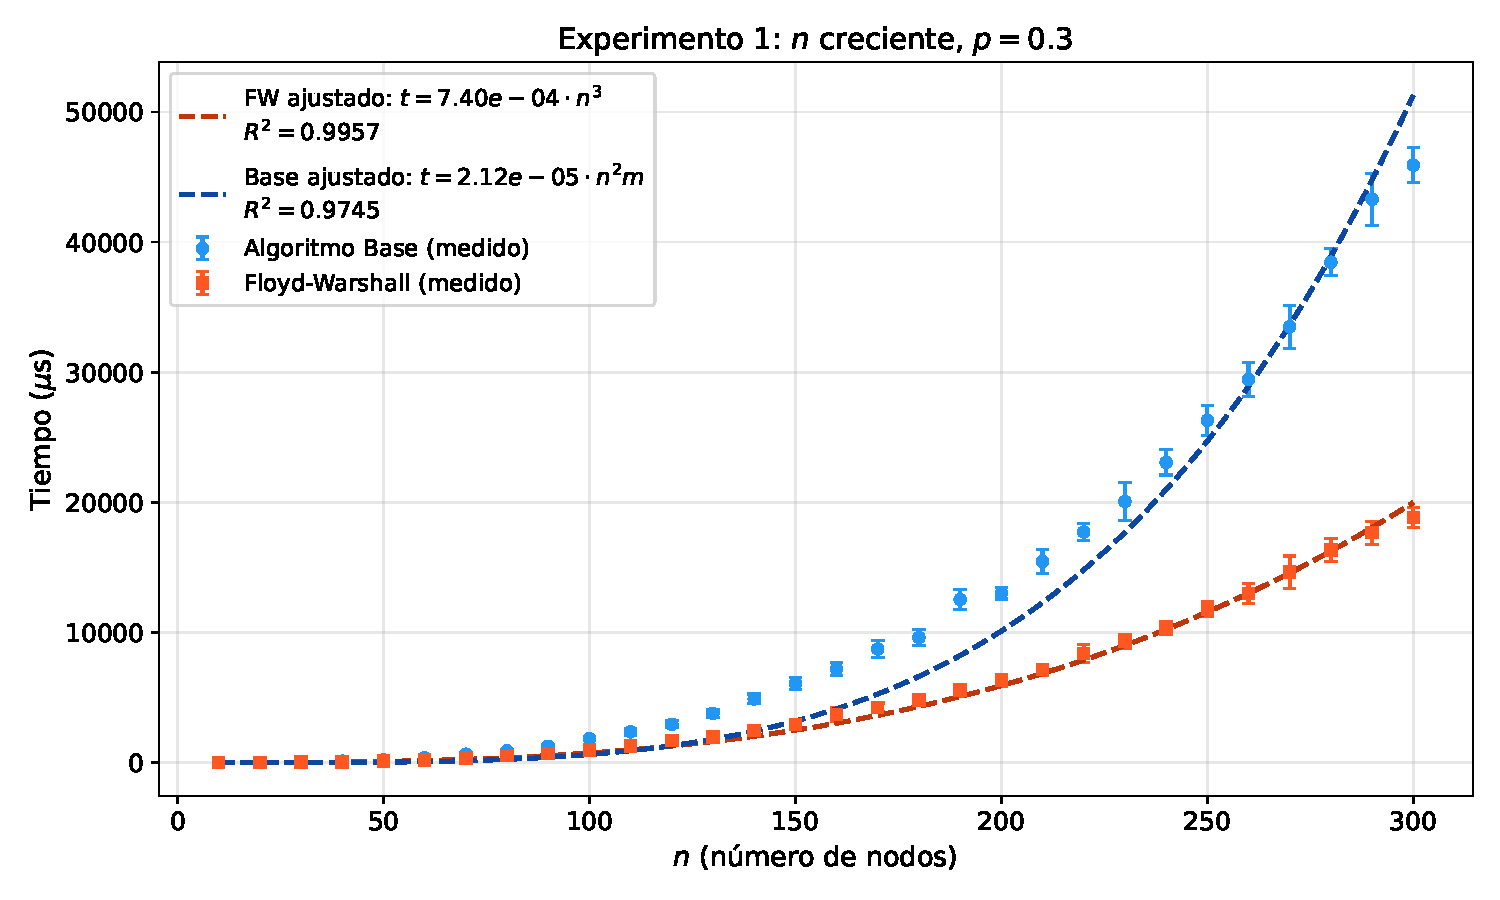
\includegraphics[width=0.95\textwidth]{../experimentos/resultados/graficos/e1_n_creciente.pdf}
\caption{Experimento 1: $n$ creciente, $p=0.3$. Floyd-Warshall escala como
$n^3$; el Algoritmo Base como $n^4$. Las curvas punteadas son los ajustes por
mínimos cuadrados.}
\label{fig:e1}
\end{figure}

\pagebreak

\subsection{Experimento 2: densidad creciente con $n$ fijo}

\textbf{Parámetros:} $n=100$ fijo, $p\in[0.1,1.0]$ con step $0.1$, pesos en
$[0,10]$, 64~runs por punto.

Con $n=100$, Floyd-Warshall ejecuta $\Theta(100^3)$ operaciones
independientemente de $m$, por lo que su tiempo debe ser aproximadamente
constante. El Algoritmo Base escala como $O(n^2m)=O(10^4\cdot m)$, es decir
lineal en $m$. La Figura~\ref{fig:e2} confirma ambas predicciones.
Código fuente: Anexo~\ref{app:exp2}.

\begin{figure}[H]
\centering
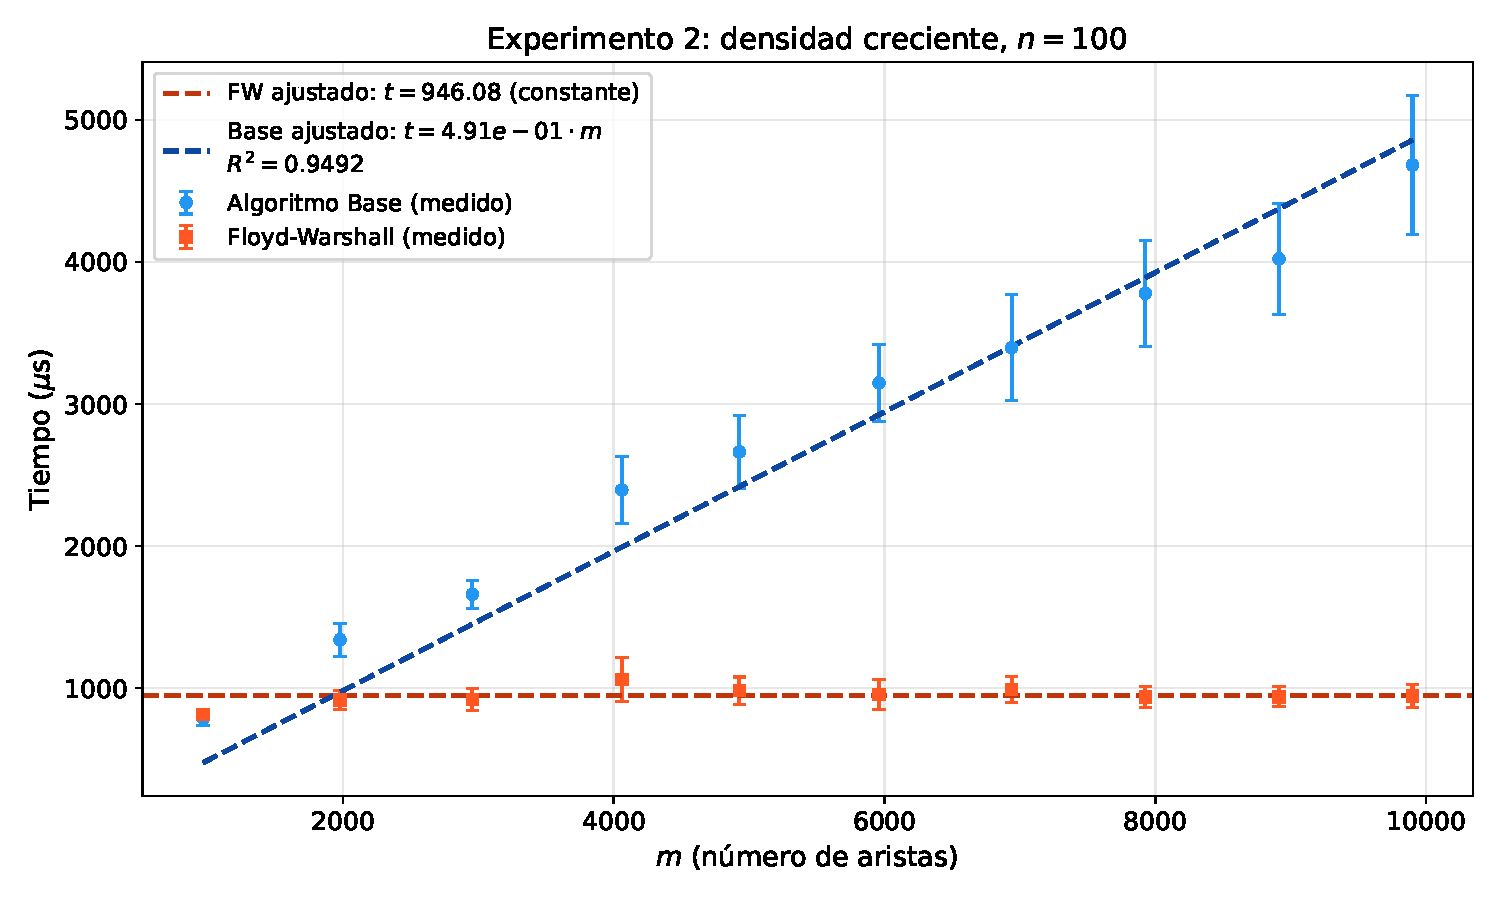
\includegraphics[width=0.95\textwidth]{../experimentos/resultados/graficos/e2_densidad.pdf}
\caption{Experimento 2: densidad creciente, $n=100$ fijo. Floyd-Warshall es
constante; el Algoritmo Base crece linealmente con $m$.}
\label{fig:e2}
\end{figure}

\pagebreak

\subsection{Experimento 3: pesos negativos}

\textbf{Parámetros:} $p=0.15$, pesos en $[-2,10]$, $n\in[10,200]$ con step
$20$, 32~runs por punto.

Los pesos incluyen valores negativos para evaluar su impacto en el tiempo
de Bellman-Ford. La densidad $p=0.15$ se eligió como balance: con
densidades mayores el Algoritmo Base se volvía demasiado lento incluso con
\texttt{-O2}, mientras que con densidades mucho menores los grafos resultaban
demasiado dispersos y los tiempos poco significativos.
Con esta configuración la mayoría de los grafos contiene al
menos un ciclo negativo para $n\ge 55$; no se filtran porque ambos algoritmos
los detectan correctamente y porque descartar grafos con ciclos negativos
habría requerido ejecutar Floyd-Warshall repetidas veces por cada $n$ hasta
encontrar uno libre de ciclos, volviendo el experimento impracticablemente
lento para $n$ grandes.

En cuanto a los resultados, con pesos no negativos (E1) Bellman-Ford suele
alcanzar el punto fijo en pocas rondas y el early exit corta la ejecución;
con pesos negativos, una arista negativa puede seguir mejorando distancias
durante muchas más rondas (a veces las $n-1$ completas), lo que anula el
early exit y dispara el tiempo. Floyd-Warshall, en cambio, es insensible al
signo de los pesos y ejecuta exactamente $n^3$ iteraciones en todos los
casos. La Figura~\ref{fig:e3} muestra que, a diferencia del Experimento~1,
la brecha entre ambos algoritmos se amplía significativamente por este
efecto. Código fuente: Anexo~\ref{app:exp3}.

\begin{figure}[H]
\centering
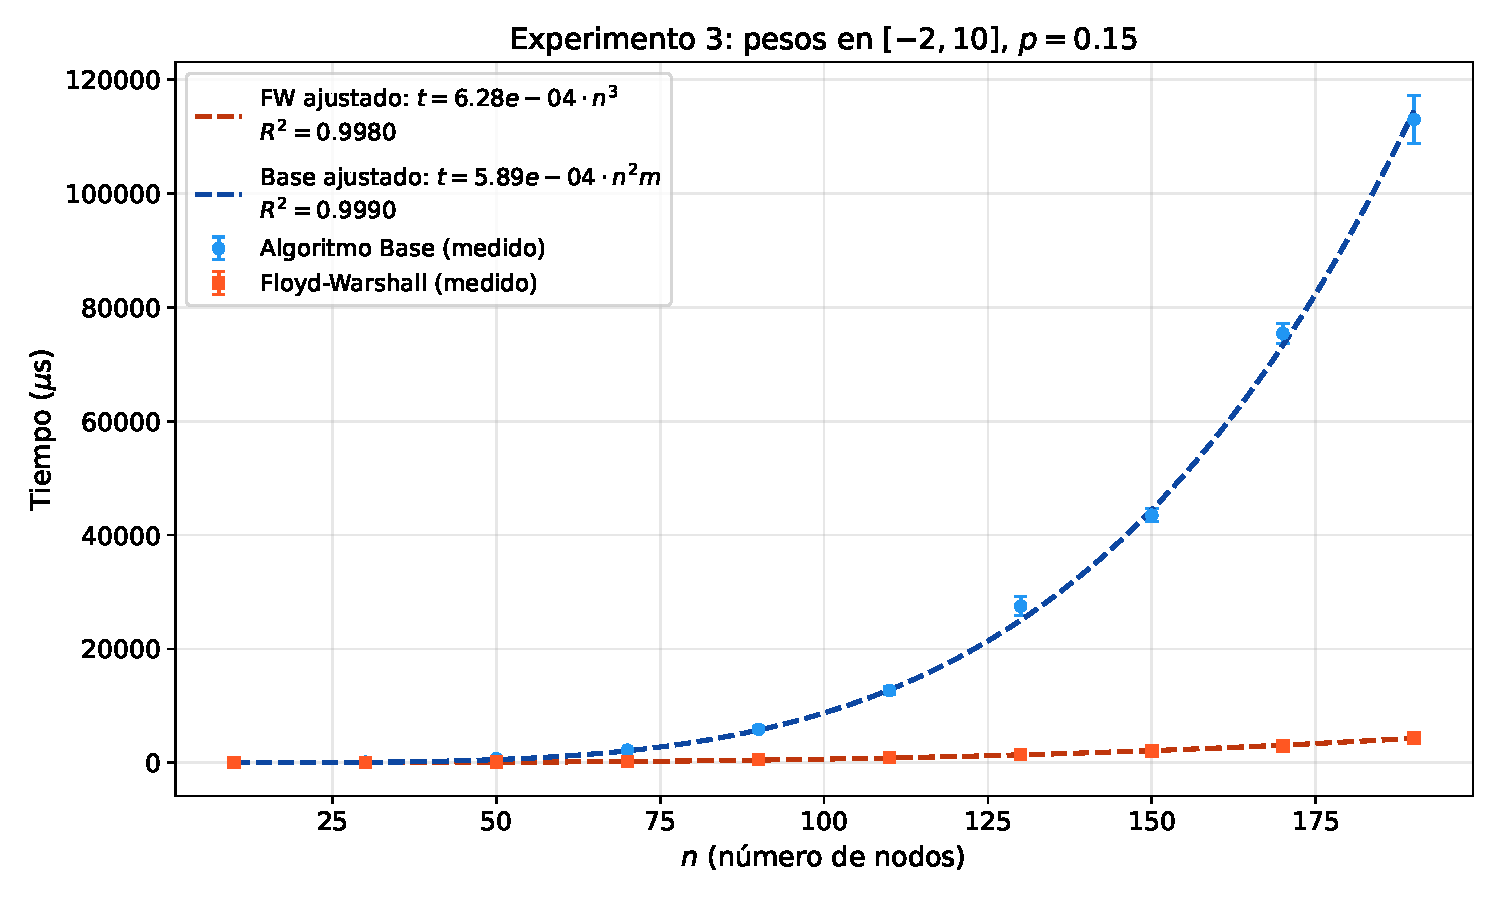
\includegraphics[width=0.95\textwidth]{../experimentos/resultados/graficos/e3_pesos_negativos.pdf}
\caption{Experimento 3: pesos en $[-2,10]$, $p=0.15$. Los pesos negativos
anulan el early exit de Bellman-Ford y amplían la brecha con Floyd-Warshall.}
\label{fig:e3}
\end{figure}

\pagebreak

\subsection{Experimento 4: grafos completos}

\textbf{Parámetros:} $p=1.0$ (grafo completo, $m=n(n-1)$), pesos en
$[0,10]$, $n\in[10,200]$ con step $20$, 32~runs por punto.

Este es el peor caso asintótico para el Algoritmo Base: con
$m=n(n-1)=\Theta(n^2)$, su complejidad se vuelve $O(n^4)$ pura, mientras que
Floyd-Warshall se mantiene en $\Theta(n^3)$. La brecha entre ambos es máxima,
como ilustra la Figura~\ref{fig:e4}.
Código fuente: Anexo~\ref{app:exp4}.

\begin{figure}[H]
\centering
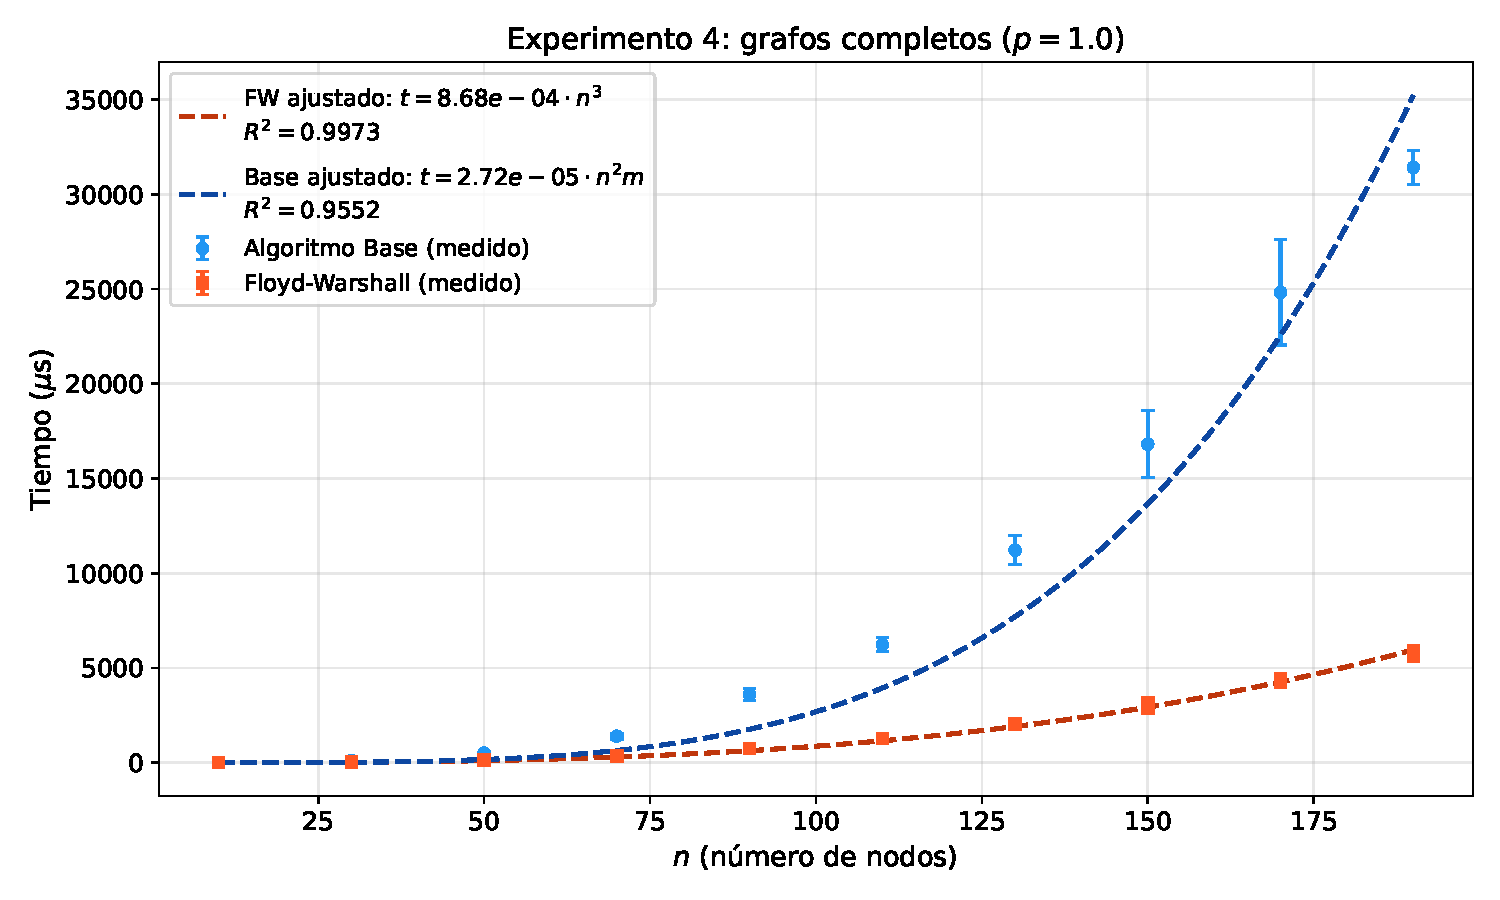
\includegraphics[width=0.95\textwidth]{../experimentos/resultados/graficos/e4_grafos_completos.pdf}
\caption{Experimento 4: grafos completos ($p=1.0$). La brecha $O(n^4)$ vs.\
$\Theta(n^3)$ es máxima.}
\label{fig:e4}
\end{figure}

\subsection{Generación de los gráficos}

Los gráficos fueron generados con Python~3 (matplotlib) mediante el script
\texttt{experimentos/graficar.py}. Cada gráfico incluye los puntos medidos
con barras de error ($\pm 1$ desviación estándar) y las curvas de ajuste
teórico calculadas por mínimos cuadrados con intercepto nulo; el coeficiente
de determinación $R^2$ se reporta en la leyenda.

\pagebreak

% ==============================================================================
\section{Datasets reales (pregunta 2.3)}
\label{sec:datasets}

Se ejecutó Floyd-Warshall sobre dos datasets reales obtenidos de
Network Repository \cite{networkrepository}. La Tabla~\ref{tab:datasets}
resume los resultados. Las matrices de distancia completas se escribieron en
archivos CSV con formato \texttt{nodo1,nodo2,distancia}, donde la distancia
es \texttt{INF} si no existe camino entre el par.

\begin{table}[ht]
\centering
\begin{tabular}{lrrrc}
\toprule
Dataset & $n$ & $m$ & Tiempo (s) & Ciclo negativo \\
\midrule
\texttt{bio-SC-TS} & 636 & 3\,959 & 0.125 & No \\
\texttt{power-685-bus} & 685 & 3\,249 & 0.157 & Sí \\
\bottomrule
\end{tabular}
\caption{Resultados de Floyd-Warshall sobre datasets reales.}
\label{tab:datasets}
\end{table}

\texttt{bio-SC-TS} es una red biológica de 636 nodos y 3\,959 aristas
(dirigida, sin pesos negativos). Floyd-Warshall procesa los
$636^3\approx 2.57\times 10^8$ pasos del bucle interno en $0.125$~s,
consistente con la complejidad $\Theta(n^3)$ y potenciado por la
compilación con \texttt{-O2}, que explota la localidad de caché del acceso
secuencial a la matriz y optimiza el bucle interno mediante register
allocation y loop unrolling.

\texttt{power-685-bus} es una matriz de admitancia de un sistema eléctrico
de 685 barras, exportada en formato Matrix~Market. Contiene pesos negativos
que producen ciclos negativos; Floyd-Warshall los detecta correctamente
($D[i][i]<0$ en la diagonal). Las entradas del CSV son mayoritariamente
\texttt{INF} porque la presencia de un ciclo negativo invalida las distancias
entre pares afectados. \linebreak
Código fuente: Anexo~\ref{app:datasets}.

% ==============================================================================
\section{Discusión y Extensiones}
\label{sec:discusion}

\subsection{Discusión de los resultados experimentales (pregunta 3.1)}

Los experimentos muestran una correspondencia clara entre la teoría y la
ejecución práctica. En todos los casos las curvas de ajuste obtienen
coeficientes $R^2$ cercanos a~1, lo que confirma que las cotas asintóticas
$O(n^2m)$ para el Algoritmo Base y $\Theta(n^3)$ para Floyd-Warshall predicen
correctamente el comportamiento observado.

Sin embargo, se aprecian varios fenómenos que la notación asintótica no captura:

\begin{enumerate}
  \item \textbf{Constante multiplicativa y localidad de caché.} En el
  Experimento~1, Floyd-Warshall es consistentemente más rápido que el
  Algoritmo Base incluso para los $n$ más pequeños, donde la diferencia
  asintótica aún no domina. Esto se debe a que el bucle interno de
  Floyd-Warshall solo realiza una suma, una comparación y una asignación
  sobre una matriz contigua en memoria (excelente localidad de caché),
  mientras que el Algoritmo Base recorre la lista de aristas $n$ veces, con
  patrones de acceso a memoria menos regulares.

  \item \textbf{Pesos negativos y early exit.} En el Experimento~3, la brecha
  entre ambos algoritmos es mucho mayor que en el Experimento~1. La causa es
  que Bellman-Ford implementa un early exit cuando una ronda completa no
  produce ninguna relajación. Con pesos no negativos, esto ocurre tras pocas
  rondas; con pesos negativos, el algoritmo suele necesitar las $n-1$ rondas
  completas, perdiendo esa optimización. Floyd-Warshall no tiene este
  mecanismo y su tiempo es independiente del signo de los pesos.

  \item \textbf{Efectos de caché.} En el Experimento~2, el tiempo de
  Floyd-Warshall no es perfectamente constante: muestra una ligera tendencia
  creciente con $m$. Esto no contradice $\Theta(n^3)$ (que es independiente
  de $m$ asintóticamente), pero refleja que la construcción de $D^{(0)}$
  depende de $m$ y que un mayor número de aristas puede afectar la
  localidad de los accesos durante las primeras iteraciones.

  \item \textbf{Impacto de la optimización del compilador.} Para verificar
  que la elección de \texttt{-O2} era la correcta, se repitieron todos los
  experimentos con \texttt{-O0} (la bandera sugerida por uhr). La diferencia
  es contundente: Floyd-Warshall es entre 14 y 33 veces más rápido con
  \texttt{-O2}, mientras que el Algoritmo Base apenas cambia (Tabla~%
  \ref{tab:o2vso0}). Esto se debe a que el triple bucle de Floyd-Warshall
  sobre una matriz contigua es el caso ideal para loop unrolling, register
  allocation y vectorización; el Algoritmo Base, que recorre una lista de
  aristas con accesos impredecibles a memoria, no se beneficia de estas
  optimizaciones. Medir con \texttt{-O0} habría distorsionado la comparación
  al eliminar artificialmente una de las ventajas prácticas más importantes
  de Floyd-Warshall.

  \begin{table}[ht]
  \centering
  \begin{tabular}{lrrr}
  \toprule
  Experimento & FW con \texttt{-O0} & FW con \texttt{-O2} & Factor \\
  \midrule
  E1 (coef.\ $n^3$)            & $1.35\times10^{-2}$ & $7.40\times10^{-4}$ & 18$\times$ \\
  E2 (constante, $\mu$s)       & 13\,260 & 946    & 14$\times$ \\
  E3 (coef.\ $n^3$)            & $2.11\times10^{-2}$ & $6.28\times10^{-4}$ & 33$\times$ \\
  E4 (coef.\ $n^3$)            & $1.46\times10^{-2}$ & $8.68\times10^{-4}$ & 17$\times$ \\
  \bottomrule
  \end{tabular}
  \caption{Comparación de Floyd-Warshall con \texttt{-O0} vs.\ \texttt{-O2}.
  En E2 se compara la constante del ajuste; en E3 y E4 el coeficiente de
  $n^3$.}
  \label{tab:o2vso0}
  \end{table}
\end{enumerate}

\subsection{Caso especial: pesos unitarios y otros contextos (pregunta 3.2)}

\textbf{Pesos unitarios.} Si todos los pesos de las aristas son $1$, el
problema APSP se reduce a calcular la distancia (en número de aristas) entre
todo par de nodos. En este caso existe una solución más rápida que
Floyd-Warshall: ejecutar BFS desde cada nodo. Como BFS sobre un grafo no
pesado cuesta $O(n+m)$, las $n$ ejecuciones suman $O(n(n+m))=O(n^2+nm)$.
En grafos dispersos ($m=O(n)$) esto es $O(n^2)$, un factor $n$ mejor que
Floyd-Warshall; en grafos densos ($m=\Theta(n^2)$) es $O(n^3)$, igual
asintóticamente pero con mejores constantes (BFS usa colas, no aritmética de
punto flotante).

\textbf{Otros contextos donde se puede superar a Floyd-Warshall.}
\begin{itemize}
  \item \textbf{Grafos dispersos} ($m=O(n)$): el Algoritmo Base ya es
  $O(n^3)$ como Floyd-Warshall, pero ejecutar Dijkstra desde cada nodo
  (con pesos no negativos) da $O(n(m+n\log n))$, que en grafos dispersos es
  $O(n^2\log n)$, mejor que $O(n^3)$.
  \item \textbf{Grafos sin ciclos} (DAGs): APSP se resuelve en
  $O(n(n+m))=O(n^2+nm)$ mediante orden topológico y programación dinámica.
  \item \textbf{Matrices de adyacencia densas con pesos pequeños}: el
  algoritmo de Williams \cite{williams2014} resuelve APSP en
  $\tilde{O}(n^3/\log^2 n)$ usando el Method of Four Russians sobre el
  semianillo $(\min,+)$.
\end{itemize}

\subsection{Complejidad asintótica conocida y uso práctico (pregunta 3.3)}

\textbf{Mejor complejidad asintótica conocida.} Para el problema APSP
general (con pesos reales arbitrarios), el mejor algoritmo conocido a la
fecha es el de Williams~\cite{williams2014}, que alcanza tiempo
$\tilde{O}(n^3 / \log^2 n)$ mediante una combinación de las técnicas de
Valiant (multiplicación de matrices sobre el semianillo $(\min,+)$) y el
método de los four russians. No se conoce un algoritmo subcúbico
verdaderamente general (i.e., $O(n^{3-\varepsilon})$ para $\varepsilon>0$)
para APSP con pesos reales; de hecho, la hipótesis del APSP conjetura que no
existe.

Para grafos con pesos enteros pequeños (en valor absoluto acotado por $M$),
existen algoritmos verdaderamente subcúbicos: Zwick~\cite{zwick2002} da
$\tilde{O}(Mn^{\omega})$, donde $\omega<2.372$ es el exponente de la
multiplicación de matrices, aprovechando la reducción de APSP a
multiplicación de matrices sobre $(\min,+)$.

\textbf{Implementación en la práctica.} En librerías reales de grafos, la
versión que se utiliza no es la ingenua de triple bucle, sino una variante
\emph{bloqueada} (blocked Floyd-Warshall) que divide la matriz en bloques
que caben en la caché L2/L3 del procesador, explotando al máximo la localidad
espacial y temporal. Librerías como Boost Graph Library (C++) delegan APSP a
$n$ ejecuciones de Dijkstra cuando los pesos son no negativos y el grafo es
disperso, reservando Floyd-Warshall bloqueado para grafos densos o cuando se
requiere el camino más corto entre \emph{todos} los pares sin excepción.

\pagebreak
\appendix
\section{Códigos fuente}

\subsection{\texttt{src/grafo.hpp}}\label{app:grafo}
\lstinputlisting[style=cpp]{../src/grafo.hpp}

\subsection{\texttt{src/apsp.hpp}}\label{app:apsp}
\lstinputlisting[style=cpp]{../src/apsp.hpp}
\pagebreak
\subsection{\texttt{src/verificar.cpp}}\label{app:verificar}
\lstinputlisting[style=cpp]{../src/verificar.cpp}

\subsection{\texttt{experimentos/exp1\_n\_creciente.cpp}}\label{app:exp1}
\lstinputlisting[style=cpp]{../experimentos/exp1_n_creciente.cpp}

\subsection{\texttt{experimentos/exp2\_densidad.cpp}}\label{app:exp2}
\lstinputlisting[style=cpp]{../experimentos/exp2_densidad.cpp}
\pagebreak
\subsection{\texttt{experimentos/exp3\_pesos\_negativos.cpp}}\label{app:exp3}
\lstinputlisting[style=cpp]{../experimentos/exp3_pesos_negativos.cpp}

\subsection{\texttt{experimentos/exp4\_grafos\_completos.cpp}}\label{app:exp4}
\lstinputlisting[style=cpp]{../experimentos/exp4_grafos_completos.cpp}

\subsection{\texttt{experimentos/datasets\_reales.cpp}}\label{app:datasets}
\lstinputlisting[style=cpp]{../experimentos/datasets_reales.cpp}

\begin{thebibliography}{2}
\bibitem{clrs} T.~H. Cormen, C.~E. Leiserson, R.~L. Rivest y C.~Stein,
\emph{Introduction to Algorithms}, 3.\textsuperscript{a}~ed., MIT Press,
2009. Capítulos 24 y 25.

\bibitem{networkrepository}
R.~A. Rossi y N.~K. Ahmed, ``The Network Data Repository with Interactive
Graph Analytics and Visualization,'' en \emph{Proc.\ 29th AAAI Conf.\
Artificial Intelligence}, 2015. \url{https://networkrepository.com}

\bibitem{williams2014}
R.~Williams, ``Faster all-pairs shortest paths via circuit complexity,''
en \emph{Proc.\ 46th ACM Symp.\ Theory of Computing (STOC)}, pp.~664--673,
2014.

\bibitem{zwick2002}
U.~Zwick, ``All pairs shortest paths using bridging sets and rectangular
matrix multiplication,'' \emph{Journal of the ACM}, vol.~49, no.~3,
pp.~289--317, 2002.
\end{thebibliography}

\end{document}
